\documentclass[a4paper, 12pt]{article}

% ~~~~~~~~~~~~~~~~~~~~~~~~~~~~~~~~~~~~~~~~
% ~~~~~~~~~~~~~~~ PACKAGES ~~~~~~~~~~~~~~~
% ~~~~~~~~~~~~~~~~~~~~~~~~~~~~~~~~~~~~~~~~

\usepackage{relsize}
\usepackage{amsmath}
\usepackage{tikz}
\usepackage{xcolor}
\usetikzlibrary{arrows}
\usetikzlibrary{positioning}

% ~~~~~~~~~~~~~~~~~~~~~~~~~~~~~~~~~~~~~~~~
% ~~~~~~~~~~~~~~~ PREAMBLE ~~~~~~~~~~~~~~~
% ~~~~~~~~~~~~~~~~~~~~~~~~~~~~~~~~~~~~~~~~

\title{Demo Document No. 1\\[0.4em]\smaller{for the SEPTeX module}}
\author{Marcel Simader}
\date{}
\pagenumbering{gobble}
% This is indeed a comment in the preamble

% ~~~~~~~~~~~~~~~~~~~~~~~~~~~~~~~~~~~~
% ~~~~~~~~~~~~~~~ BODY ~~~~~~~~~~~~~~~
% ~~~~~~~~~~~~~~~~~~~~~~~~~~~~~~~~~~~~

\begin{document}
	\maketitle
	
	\noindent This is some text, and it contains a potentially % confusing comment for the "soft" line 
		% wrap % functionality
	
	And this is some text that goes on and on and on and on and on and on and on and on and on and on 
		and on and on and on and on and on and on and on and on and on and on and on\ldots
	This is a \LaTeX\ sentence -- wow!
	\begin{gather*}
		\left[ 1, \frac{1}{3}, 3, \text{abc} \right]
		\left\{ 1, abc, -\frac{3}{5}, -\frac{2}{7} \right\}
		\\
		\left( \left\{ 1, 2, 3, -\frac{9}{2} \right\}, \text{add} \right)
		\left( \left\{ 1, 2, 3, -\frac{9}{2} \right\}, \text{add}, \text{multiply} \right)
	\end{gather*}
	
	\newpage
	
	\begin{figure}[h!]
		\begin{center}
			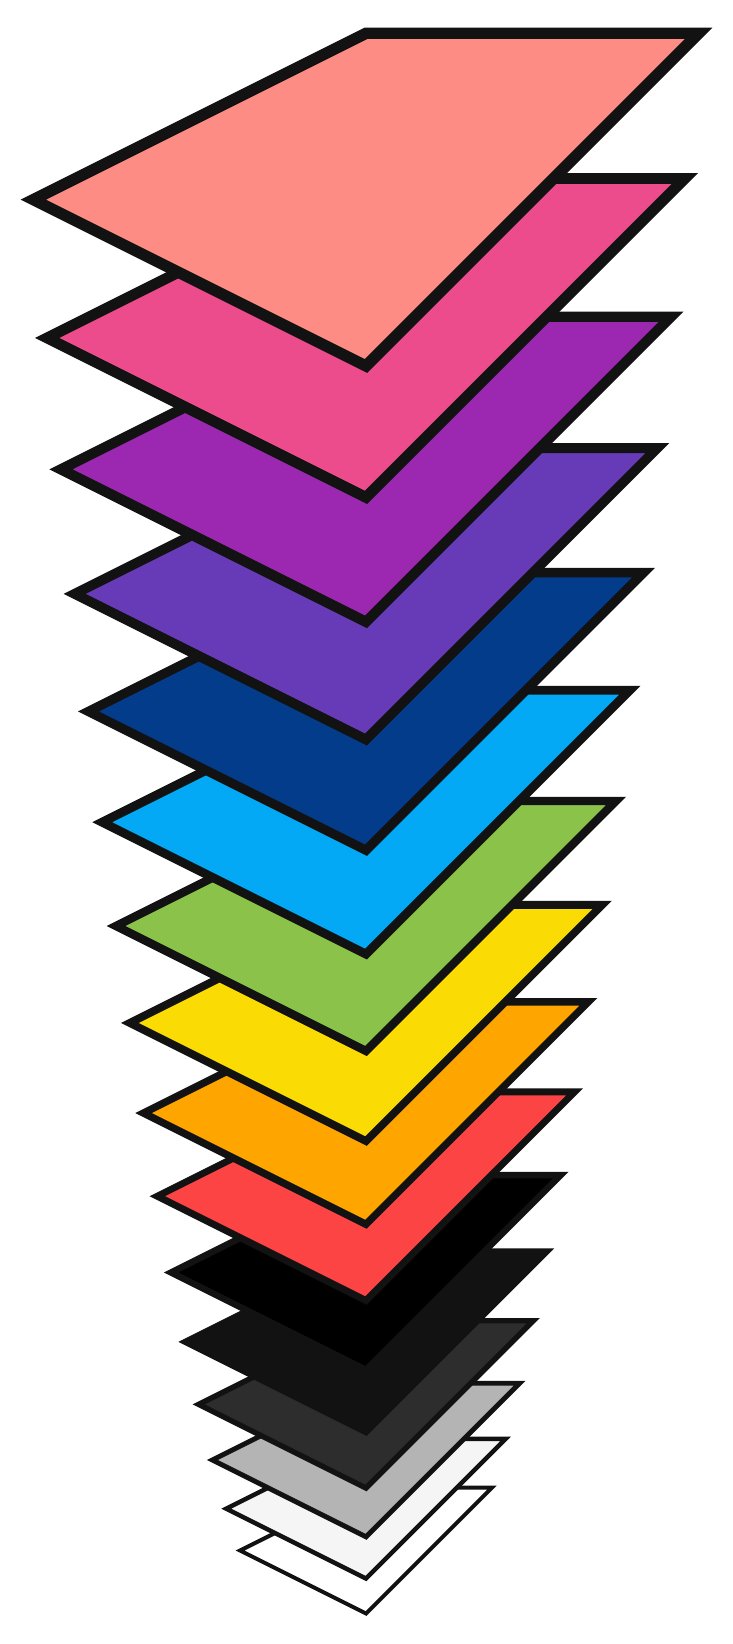
\begin{tikzpicture}[draw]
				\definecolor{WHITE}{RGB}{255, 255, 255}
				\definecolor{ALMOST_WHITE}{RGB}{245, 245, 245}
				\definecolor{LIGHT_GRAY}{RGB}{180, 180, 180}
				\definecolor{DARK_GRAY}{RGB}{45, 45, 45}
				\definecolor{ALMOST_BLACK}{RGB}{18, 18, 18}
				\definecolor{BLACK}{RGB}{0, 0, 0}
				\definecolor{RED}{RGB}{252, 68, 68}
				\definecolor{ORANGE}{RGB}{255, 165, 0}
				\definecolor{YELLOW}{RGB}{251, 219, 4}
				\definecolor{GREEN}{RGB}{139, 195, 74}
				\definecolor{LIGHT_BLUE}{RGB}{3, 169, 244}
				\definecolor{DARK_BLUE}{RGB}{4, 60, 140}
				\definecolor{PURPLE}{RGB}{103, 58, 183}
				\definecolor{MAGENTA}{RGB}{156, 39, 176}
				\definecolor{PINK}{RGB}{236, 76, 140}
				\definecolor{ROSE}{RGB}{252, 140, 132}
				\begin{scope}[draw, scale={0.4}]
					\draw[draw, line width={0.5mm}, color={ALMOST_BLACK!100}, fill={WHITE!100}] ( 0.0000000, 
						0.0000000) -- ( 4.0000000,  4.0000000) -- ( 0.0000000,  4.0000000) -- (-4.0000000, 
						2.0000000) -- cycle;
				\end{scope}
				
				\begin{scope}[draw, scale={0.44375000000000003}]
					\draw[draw, line width={0.5625mm}, color={ALMOST_BLACK!100}, fill={ALMOST_WHITE!100}] 
						( 0.0000000,  1.0000000) -- ( 4.0000000,  5.0000000) -- ( 0.0000000,  5.0000000) 
						-- (-4.0000000,  3.0000000) -- cycle;
				\end{scope}
				
				\begin{scope}[draw, scale={0.48750000000000004}]
					\draw[draw, line width={0.625mm}, color={ALMOST_BLACK!100}, fill={LIGHT_GRAY!100}] 
						( 0.0000000,  2.0000000) -- ( 4.0000000,  6.0000000) -- ( 0.0000000,  6.0000000) 
						-- (-4.0000000,  4.0000000) -- cycle;
				\end{scope}
				
				\begin{scope}[draw, scale={0.53125}]
					\draw[draw, line width={0.6875mm}, color={ALMOST_BLACK!100}, fill={DARK_GRAY!100}] 
						( 0.0000000,  3.0000000) -- ( 4.0000000,  7.0000000) -- ( 0.0000000,  7.0000000) 
						-- (-4.0000000,  5.0000000) -- cycle;
				\end{scope}
				
				\begin{scope}[draw, scale={0.575}]
					\draw[draw, line width={0.75mm}, color={ALMOST_BLACK!100}, fill={ALMOST_BLACK!100}] 
						( 0.0000000,  4.0000000) -- ( 4.0000000,  8.0000000) -- ( 0.0000000,  8.0000000) 
						-- (-4.0000000,  6.0000000) -- cycle;
				\end{scope}
				
				\begin{scope}[draw, scale={0.61875}]
					\draw[draw, line width={0.8125mm}, color={ALMOST_BLACK!100}, fill={BLACK!100}] ( 
						0.0000000,  5.0000000) -- ( 4.0000000,  9.0000000) -- ( 0.0000000,  9.0000000) 
						-- (-4.0000000,  7.0000000) -- cycle;
				\end{scope}
				
				\begin{scope}[draw, scale={0.6625}]
					\draw[draw, line width={0.875mm}, color={ALMOST_BLACK!100}, fill={RED!100}] ( 0.0000000, 
						6.0000000) -- ( 4.0000000,  10.0000000) -- ( 0.0000000,  10.0000000) -- (-4.0000000, 
						8.0000000) -- cycle;
				\end{scope}
				
				\begin{scope}[draw, scale={0.70625}]
					\draw[draw, line width={0.9375mm}, color={ALMOST_BLACK!100}, fill={ORANGE!100}] ( 
						0.0000000,  7.0000000) -- ( 4.0000000,  11.0000000) -- ( 0.0000000,  11.0000000) 
						-- (-4.0000000,  9.0000000) -- cycle;
				\end{scope}
				
				\begin{scope}[draw, scale={0.75}]
					\draw[draw, line width={1.0mm}, color={ALMOST_BLACK!100}, fill={YELLOW!100}] ( 0.0000000, 
						8.0000000) -- ( 4.0000000,  12.0000000) -- ( 0.0000000,  12.0000000) -- (-4.0000000, 
						10.0000000) -- cycle;
				\end{scope}
				
				\begin{scope}[draw, scale={0.79375}]
					\draw[draw, line width={1.0625mm}, color={ALMOST_BLACK!100}, fill={GREEN!100}] ( 
						0.0000000,  9.0000000) -- ( 4.0000000,  13.0000000) -- ( 0.0000000,  13.0000000) 
						-- (-4.0000000,  11.0000000) -- cycle;
				\end{scope}
				
				\begin{scope}[draw, scale={0.8375}]
					\draw[draw, line width={1.125mm}, color={ALMOST_BLACK!100}, fill={LIGHT_BLUE!100}] 
						( 0.0000000,  10.0000000) -- ( 4.0000000,  14.0000000) -- ( 0.0000000,  14.0000000) 
						-- (-4.0000000,  12.0000000) -- cycle;
				\end{scope}
				
				\begin{scope}[draw, scale={0.88125}]
					\draw[draw, line width={1.1875mm}, color={ALMOST_BLACK!100}, fill={DARK_BLUE!100}] 
						( 0.0000000,  11.0000000) -- ( 4.0000000,  15.0000000) -- ( 0.0000000,  15.0000000) 
						-- (-4.0000000,  13.0000000) -- cycle;
				\end{scope}
				
				\begin{scope}[draw, scale={0.9249999999999999}]
					\draw[draw, line width={1.25mm}, color={ALMOST_BLACK!100}, fill={PURPLE!100}] ( 0.0000000, 
						12.0000000) -- ( 4.0000000,  16.0000000) -- ( 0.0000000,  16.0000000) -- (-4.0000000, 
						14.0000000) -- cycle;
				\end{scope}
				
				\begin{scope}[draw, scale={0.96875}]
					\draw[draw, line width={1.3125mm}, color={ALMOST_BLACK!100}, fill={MAGENTA!100}] 
						( 0.0000000,  13.0000000) -- ( 4.0000000,  17.0000000) -- ( 0.0000000,  17.0000000) 
						-- (-4.0000000,  15.0000000) -- cycle;
				\end{scope}
				
				\begin{scope}[draw, scale={1.0125}]
					\draw[draw, line width={1.375mm}, color={ALMOST_BLACK!100}, fill={PINK!100}] ( 0.0000000, 
						14.0000000) -- ( 4.0000000,  18.0000000) -- ( 0.0000000,  18.0000000) -- (-4.0000000, 
						16.0000000) -- cycle;
				\end{scope}
				
				\begin{scope}[draw, scale={1.05625}]
					\draw[draw, line width={1.4375mm}, color={ALMOST_BLACK!100}, fill={ROSE!100}] ( 0.0000000, 
						15.0000000) -- ( 4.0000000,  19.0000000) -- ( 0.0000000,  19.0000000) -- (-4.0000000, 
						17.0000000) -- cycle;
				\end{scope}
				
			\end{tikzpicture}
			
		\end{center}
		
		\caption{Captions, Figures, and the Default Colors.}
	\end{figure}
	
	\newpage
	
	\begin{figure}[h!]
		\begin{center}
			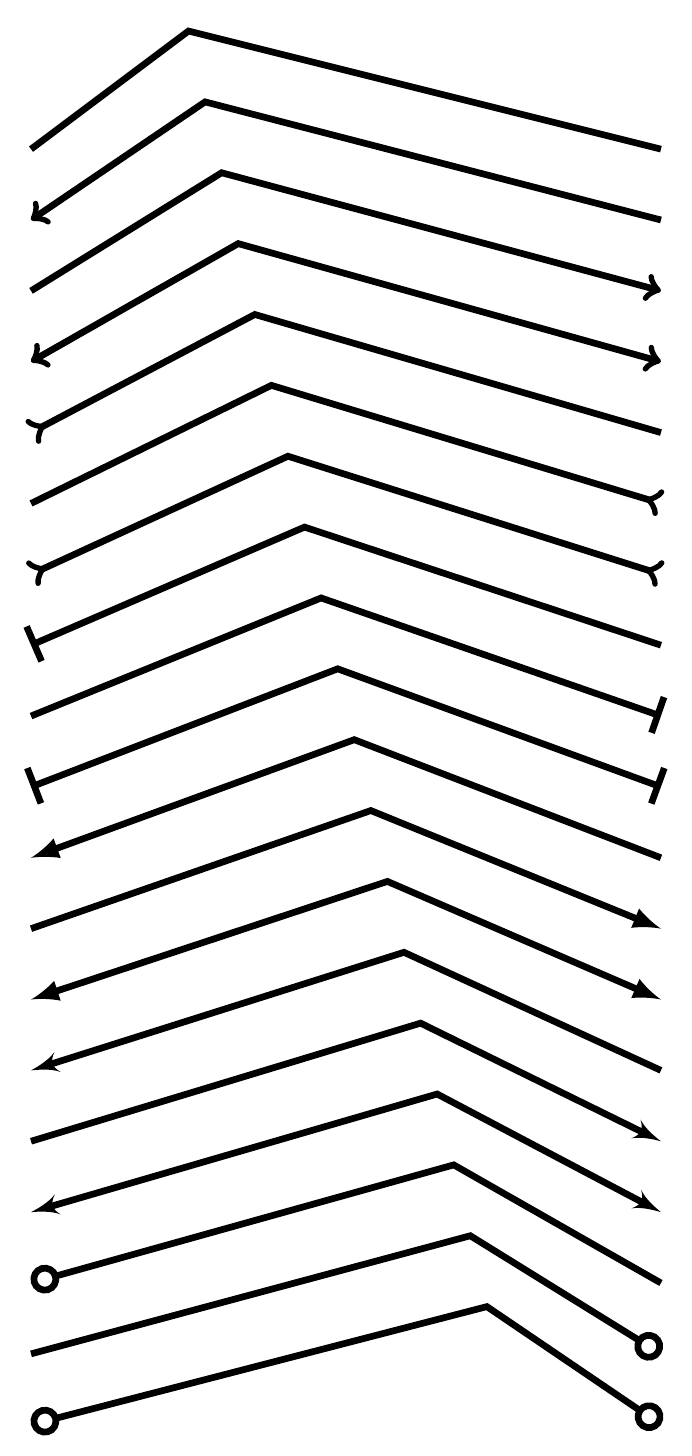
\begin{tikzpicture}[draw]
				\begin{scope}[draw, scale={2}, shift={(0, 0.0)}]
					\draw[-, draw, line width={0.85mm}] ( 0.0000000,  0.0000000) to ( 1.0000000,  0.7500000) 
						to ( 4.0000000,  0.0000000);
				\end{scope}
				
				\begin{scope}[draw, scale={2}, shift={(0, -0.45)}]
					\draw[<-, draw, line width={0.85mm}] ( 0.0000000,  0.0000000) to ( 1.1052632,  0.7500000) 
						to ( 4.0000000,  0.0000000);
				\end{scope}
				
				\begin{scope}[draw, scale={2}, shift={(0, -0.9)}]
					\draw[->, draw, line width={0.85mm}] ( 0.0000000,  0.0000000) to ( 1.2105263,  0.7500000) 
						to ( 4.0000000,  0.0000000);
				\end{scope}
				
				\begin{scope}[draw, scale={2}, shift={(0, -1.35)}]
					\draw[<->, draw, line width={0.85mm}] ( 0.0000000,  0.0000000) to ( 1.3157895,  0.7500000) 
						to ( 4.0000000,  0.0000000);
				\end{scope}
				
				\begin{scope}[draw, scale={2}, shift={(0, -1.8)}]
					\draw[>-, draw, line width={0.85mm}] ( 0.0000000,  0.0000000) to ( 1.4210526,  0.7500000) 
						to ( 4.0000000,  0.0000000);
				\end{scope}
				
				\begin{scope}[draw, scale={2}, shift={(0, -2.25)}]
					\draw[-<, draw, line width={0.85mm}] ( 0.0000000,  0.0000000) to ( 1.5263158,  0.7500000) 
						to ( 4.0000000,  0.0000000);
				\end{scope}
				
				\begin{scope}[draw, scale={2}, shift={(0, -2.7)}]
					\draw[>-<, draw, line width={0.85mm}] ( 0.0000000,  0.0000000) to ( 1.6315789,  0.7500000) 
						to ( 4.0000000,  0.0000000);
				\end{scope}
				
				\begin{scope}[draw, scale={2}, shift={(0, -3.15)}]
					\draw[|-, draw, line width={0.85mm}] ( 0.0000000,  0.0000000) to ( 1.7368421,  0.7500000) 
						to ( 4.0000000,  0.0000000);
				\end{scope}
				
				\begin{scope}[draw, scale={2}, shift={(0, -3.6)}]
					\draw[-|, draw, line width={0.85mm}] ( 0.0000000,  0.0000000) to ( 1.8421053,  0.7500000) 
						to ( 4.0000000,  0.0000000);
				\end{scope}
				
				\begin{scope}[draw, scale={2}, shift={(0, -4.05)}]
					\draw[|-|, draw, line width={0.85mm}] ( 0.0000000,  0.0000000) to ( 1.9473684,  0.7500000) 
						to ( 4.0000000,  0.0000000);
				\end{scope}
				
				\begin{scope}[draw, scale={2}, shift={(0, -4.5)}]
					\draw[latex-, draw, line width={0.85mm}] ( 0.0000000,  0.0000000) to ( 2.0526316, 
						0.7500000) to ( 4.0000000,  0.0000000);
				\end{scope}
				
				\begin{scope}[draw, scale={2}, shift={(0, -4.95)}]
					\draw[-latex, draw, line width={0.85mm}] ( 0.0000000,  0.0000000) to ( 2.1578947, 
						0.7500000) to ( 4.0000000,  0.0000000);
				\end{scope}
				
				\begin{scope}[draw, scale={2}, shift={(0, -5.4)}]
					\draw[latex-latex, draw, line width={0.85mm}] ( 0.0000000,  0.0000000) to ( 2.2631579, 
						0.7500000) to ( 4.0000000,  0.0000000);
				\end{scope}
				
				\begin{scope}[draw, scale={2}, shift={(0, -5.8500000000000005)}]
					\draw[latex'-, draw, line width={0.85mm}] ( 0.0000000,  0.0000000) to ( 2.3684211, 
						0.7500000) to ( 4.0000000,  0.0000000);
				\end{scope}
				
				\begin{scope}[draw, scale={2}, shift={(0, -6.3)}]
					\draw[-latex', draw, line width={0.85mm}] ( 0.0000000,  0.0000000) to ( 2.4736842, 
						0.7500000) to ( 4.0000000,  0.0000000);
				\end{scope}
				
				\begin{scope}[draw, scale={2}, shift={(0, -6.75)}]
					\draw[latex'-latex', draw, line width={0.85mm}] ( 0.0000000,  0.0000000) to ( 2.5789474, 
						0.7500000) to ( 4.0000000,  0.0000000);
				\end{scope}
				
				\begin{scope}[draw, scale={2}, shift={(0, -7.2)}]
					\draw[o-, draw, line width={0.85mm}] ( 0.0000000,  0.0000000) to ( 2.6842105,  0.7500000) 
						to ( 4.0000000,  0.0000000);
				\end{scope}
				
				\begin{scope}[draw, scale={2}, shift={(0, -7.65)}]
					\draw[-o, draw, line width={0.85mm}] ( 0.0000000,  0.0000000) to ( 2.7894737,  0.7500000) 
						to ( 4.0000000,  0.0000000);
				\end{scope}
				
				\begin{scope}[draw, scale={2}, shift={(0, -8.1)}]
					\draw[o-o, draw, line width={0.85mm}] ( 0.0000000,  0.0000000) to ( 2.8947368,  0.7500000) 
						to ( 4.0000000,  0.0000000);
				\end{scope}
				
			\end{tikzpicture}
			
		\end{center}
		
		\caption{The arrow styles.}
	\end{figure}
	
	\newpage
	
	\begin{figure}[h!]
		\begin{center}
			\begin{tikzpicture}[draw]
				\node[draw, circle] (x11) at (-2.5000000,  4.3301270) {11};
				\node[draw, circle] (x0) at ( 0.0000000,  5.0000000) {0};
				\node[draw, circle] (x1) at ( 2.5000000,  4.3301270) {1};
				\node[draw, circle] (x2) at ( 4.3301270,  2.5000000) {2};
				\node[draw, circle] (x3) at ( 5.0000000,  0.0000000) {3};
				\node[draw, circle] (x4) at ( 4.3301270, -2.5000000) {4};
				\node[draw, circle] (x5) at ( 2.5000000, -4.3301270) {5};
				\node[draw, circle] (x6) at ( 0.0000000, -5.0000000) {6};
				\node[draw, circle] (x7) at (-2.5000000, -4.3301270) {7};
				\node[draw, circle] (x8) at (-4.3301270, -2.5000000) {8};
				\node[draw, circle] (x9) at (-5.0000000, -0.0000000) {9};
				\node[draw, circle] (x10) at (-4.3301270,  2.5000000) {10};
				\draw[-latex', draw, dashed, bend left={15}, line width={0.3mm}] (x11) to (x0);
				\draw[-latex', draw, dashed, bend left={15}, line width={0.3mm}] (x0) to (x1);
				\draw[-latex', draw, dashed, bend left={15}, line width={0.3mm}] (x1) to (x2);
				\draw[-latex', draw, dashed, bend left={15}, line width={0.3mm}] (x2) to (x3);
				\draw[-latex', draw, dashed, bend left={15}, line width={0.3mm}] (x3) to (x4);
				\draw[-latex', draw, dashed, bend left={15}, line width={0.3mm}] (x4) to (x5);
				\draw[-latex', draw, dashed, bend left={15}, line width={0.3mm}] (x5) to (x6);
				\draw[-latex', draw, dashed, bend left={15}, line width={0.3mm}] (x6) to (x7);
				\draw[-latex', draw, dashed, bend left={15}, line width={0.3mm}] (x7) to (x8);
				\draw[-latex', draw, dashed, bend left={15}, line width={0.3mm}] (x8) to (x9);
				\draw[-latex', draw, dashed, bend left={15}, line width={0.3mm}] (x9) to (x10);
				\draw[-latex', draw, dashed, bend left={15}, line width={0.3mm}] (x10) to (x11);
				\draw[-o, draw] (x0) to (x7);
			\end{tikzpicture}
			
		\end{center}
		
		\caption{Nodes, and directed paths -- wow!}
	\end{figure}
	
	\newpage
	
	\begin{figure}[h!]
		\begin{center}
			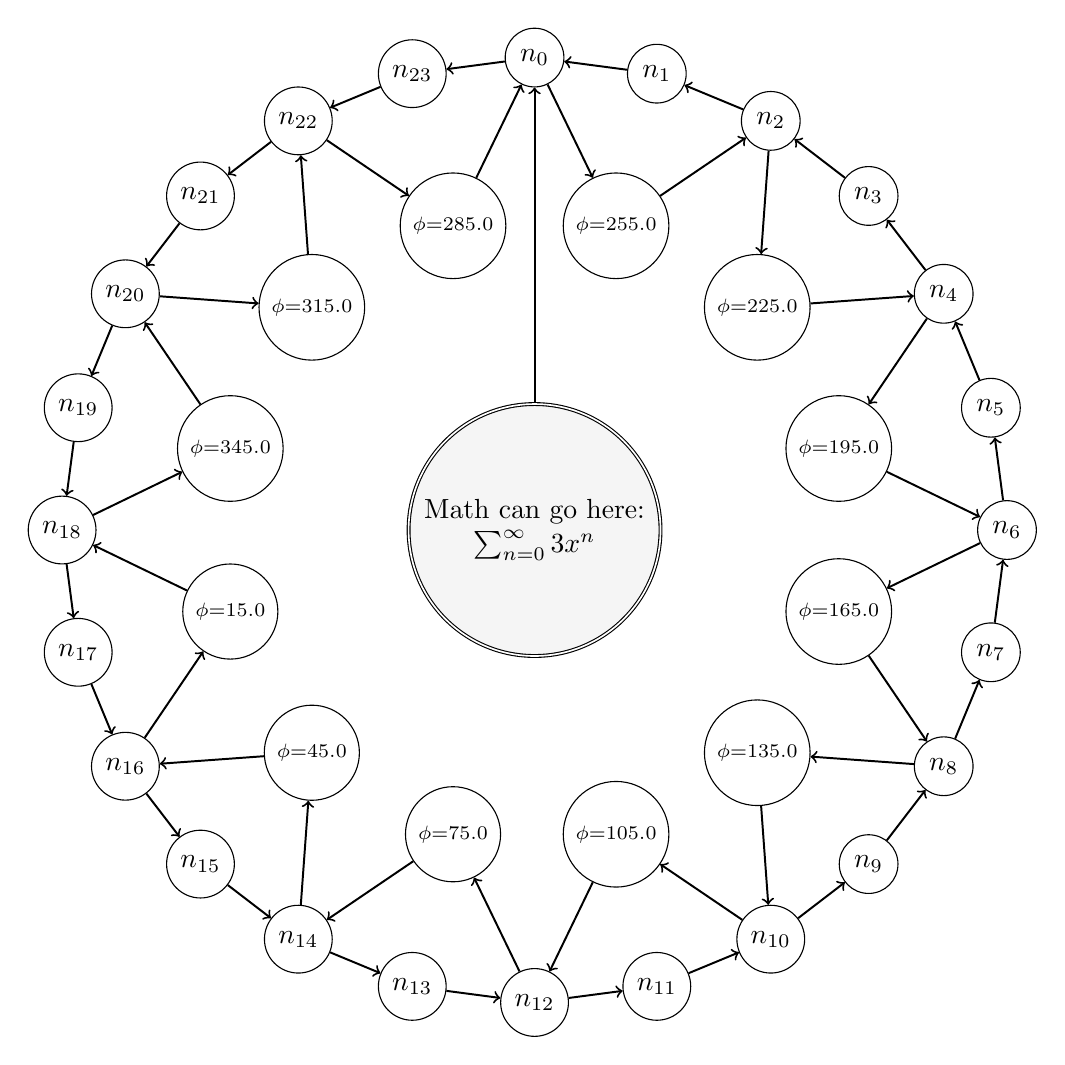
\begin{tikzpicture}[draw]
				\node[draw, circle] (y0) at ( 90.0000000: 6.0000000) {$n_{0}$};
				\definecolor{ALMOST_WHITE}{RGB}{245, 245, 245}
				\node[draw, circle, double, fill={ALMOST_WHITE!100}, align={center}] (o) at ( 0.0000000, 
					0.0000000) {Math can go here: \\$\sum_{n=0}^{\infty} 3x^n$};
				\node[draw, circle] (l1) at ( 1.0352762,  3.8637033) {$\scriptstyle \phi = 255.0$};
				\node[draw, circle] (y2) at ( 60.0000000: 6.0000000) {$n_{2}$};
				\node[draw, circle] (l3) at ( 2.8284271,  2.8284271) {$\scriptstyle \phi = 225.0$};
				\node[draw, circle] (y4) at ( 30.0000000: 6.0000000) {$n_{4}$};
				\node[draw, circle] (l5) at ( 3.8637033,  1.0352762) {$\scriptstyle \phi = 195.0$};
				\node[draw, circle] (y6) at ( 0.0000000: 6.0000000) {$n_{6}$};
				\node[draw, circle] (l7) at ( 3.8637033, -1.0352762) {$\scriptstyle \phi = 165.0$};
				\node[draw, circle] (y8) at ( 330.0000000: 6.0000000) {$n_{8}$};
				\node[draw, circle] (l9) at ( 2.8284271, -2.8284271) {$\scriptstyle \phi = 135.0$};
				\node[draw, circle] (y10) at ( 300.0000000: 6.0000000) {$n_{10}$};
				\node[draw, circle] (l11) at ( 1.0352762, -3.8637033) {$\scriptstyle \phi = 105.0$};
				\node[draw, circle] (y12) at ( 270.0000000: 6.0000000) {$n_{12}$};
				\node[draw, circle] (l13) at (-1.0352762, -3.8637033) {$\scriptstyle \phi = 75.0$};
				\node[draw, circle] (y14) at ( 240.0000000: 6.0000000) {$n_{14}$};
				\node[draw, circle] (l15) at (-2.8284271, -2.8284271) {$\scriptstyle \phi = 45.0$};
				\node[draw, circle] (y16) at ( 210.0000000: 6.0000000) {$n_{16}$};
				\node[draw, circle] (l17) at (-3.8637033, -1.0352762) {$\scriptstyle \phi = 15.0$};
				\node[draw, circle] (y18) at ( 180.0000000: 6.0000000) {$n_{18}$};
				\node[draw, circle] (l19) at (-3.8637033,  1.0352762) {$\scriptstyle \phi = 345.0$};
				\node[draw, circle] (y20) at ( 150.0000000: 6.0000000) {$n_{20}$};
				\node[draw, circle] (l21) at (-2.8284271,  2.8284271) {$\scriptstyle \phi = 315.0$};
				\node[draw, circle] (y22) at ( 120.0000000: 6.0000000) {$n_{22}$};
				\node[draw, circle] (l23) at (-1.0352762,  3.8637033) {$\scriptstyle \phi = 285.0$};
				\node[draw, circle] (y1) at ( 75.0000000: 6.0000000) {$n_{1}$};
				\node[draw, circle] (y3) at ( 45.0000000: 6.0000000) {$n_{3}$};
				\node[draw, circle] (y5) at ( 15.0000000: 6.0000000) {$n_{5}$};
				\node[draw, circle] (y7) at ( 345.0000000: 6.0000000) {$n_{7}$};
				\node[draw, circle] (y9) at ( 315.0000000: 6.0000000) {$n_{9}$};
				\node[draw, circle] (y11) at ( 285.0000000: 6.0000000) {$n_{11}$};
				\node[draw, circle] (y13) at ( 255.0000000: 6.0000000) {$n_{13}$};
				\node[draw, circle] (y15) at ( 225.0000000: 6.0000000) {$n_{15}$};
				\node[draw, circle] (y17) at ( 195.0000000: 6.0000000) {$n_{17}$};
				\node[draw, circle] (y19) at ( 165.0000000: 6.0000000) {$n_{19}$};
				\node[draw, circle] (y21) at ( 135.0000000: 6.0000000) {$n_{21}$};
				\node[draw, circle] (y23) at ( 105.0000000: 6.0000000) {$n_{23}$};
				\draw[<-, draw, line width={0.25mm}] (y0) to (o);
				\draw[<-, draw, line width={0.25mm}] (l1) to (y0);
				\draw[->, draw, line width={0.25mm}] (l1) to (y2);
				\draw[<-, draw, line width={0.25mm}] (l3) to (y2);
				\draw[->, draw, line width={0.25mm}] (l3) to (y4);
				\draw[<-, draw, line width={0.25mm}] (l5) to (y4);
				\draw[->, draw, line width={0.25mm}] (l5) to (y6);
				\draw[<-, draw, line width={0.25mm}] (l7) to (y6);
				\draw[->, draw, line width={0.25mm}] (l7) to (y8);
				\draw[<-, draw, line width={0.25mm}] (l9) to (y8);
				\draw[->, draw, line width={0.25mm}] (l9) to (y10);
				\draw[<-, draw, line width={0.25mm}] (l11) to (y10);
				\draw[->, draw, line width={0.25mm}] (l11) to (y12);
				\draw[<-, draw, line width={0.25mm}] (l13) to (y12);
				\draw[->, draw, line width={0.25mm}] (l13) to (y14);
				\draw[<-, draw, line width={0.25mm}] (l15) to (y14);
				\draw[->, draw, line width={0.25mm}] (l15) to (y16);
				\draw[<-, draw, line width={0.25mm}] (l17) to (y16);
				\draw[->, draw, line width={0.25mm}] (l17) to (y18);
				\draw[<-, draw, line width={0.25mm}] (l19) to (y18);
				\draw[->, draw, line width={0.25mm}] (l19) to (y20);
				\draw[<-, draw, line width={0.25mm}] (l21) to (y20);
				\draw[->, draw, line width={0.25mm}] (l21) to (y22);
				\draw[<-, draw, line width={0.25mm}] (l23) to (y22);
				\draw[->, draw, line width={0.25mm}] (l23) to (y0);
				\draw[<-, draw, line width={0.25mm}] (y0) to (y1);
				\draw[<-, draw, line width={0.25mm}] (y1) to (y2);
				\draw[<-, draw, line width={0.25mm}] (y2) to (y3);
				\draw[<-, draw, line width={0.25mm}] (y3) to (y4);
				\draw[<-, draw, line width={0.25mm}] (y4) to (y5);
				\draw[<-, draw, line width={0.25mm}] (y5) to (y6);
				\draw[<-, draw, line width={0.25mm}] (y6) to (y7);
				\draw[<-, draw, line width={0.25mm}] (y7) to (y8);
				\draw[<-, draw, line width={0.25mm}] (y8) to (y9);
				\draw[<-, draw, line width={0.25mm}] (y9) to (y10);
				\draw[<-, draw, line width={0.25mm}] (y10) to (y11);
				\draw[<-, draw, line width={0.25mm}] (y11) to (y12);
				\draw[<-, draw, line width={0.25mm}] (y12) to (y13);
				\draw[<-, draw, line width={0.25mm}] (y13) to (y14);
				\draw[<-, draw, line width={0.25mm}] (y14) to (y15);
				\draw[<-, draw, line width={0.25mm}] (y15) to (y16);
				\draw[<-, draw, line width={0.25mm}] (y16) to (y17);
				\draw[<-, draw, line width={0.25mm}] (y17) to (y18);
				\draw[<-, draw, line width={0.25mm}] (y18) to (y19);
				\draw[<-, draw, line width={0.25mm}] (y19) to (y20);
				\draw[<-, draw, line width={0.25mm}] (y20) to (y21);
				\draw[<-, draw, line width={0.25mm}] (y21) to (y22);
				\draw[<-, draw, line width={0.25mm}] (y22) to (y23);
				\draw[<-, draw, line width={0.25mm}] (y23) to (y0);
			\end{tikzpicture}
			
		\end{center}
		
		\caption{Graphs!}
	\end{figure}
	
\end{document}